%%%%%%%%%%%%%%%%%%%%%%%%%%%%%%%%%%%%%%
% LaTeX poster template
% Created by Nathaniel Johnston
% August 2009
% Updated by Matthew Denny: May, 2014.
% http://www.nathanieljohnston.com/index.php/2009/08/latex-poster-template/
%%%%%%%%%%%%%%%%%%%%%%%%%%%%%%%%%%%%%%

\documentclass[final]{beamer}
\usepackage{etex}
%\usepackage[size = custom,height = 121.92, width = 99.06,scale=1.1]{beamerposter}
\usepackage[size = custom,height = 99, width = 132,scale=1.1]{beamerposter}
\usepackage{graphicx}	% allows us to import images
\usepackage{natbib}
\usepackage{framed,xcolor}
\colorlet{shadecolor}{black!20}
\usepackage{tabularx}
\usepackage{multirow}
\usepackage[scriptsize]{caption}
\usepackage{amsmath}
\usepackage{amssymb,amsfonts,textcomp}
\usepackage{color,colortbl}
\usepackage{array}
\usepackage{hhline}
\usepackage{tipa}
\usepackage{relsize,exscale}
\usepackage{amsmath}
\usepackage{amssymb}
\usepackage{graphicx}
\usepackage{algcompatible}
%\usepackage{xcolor}
%\usepackage[usenames,dvipsnames]{xcolor}
\definecolor{darkgreen}{RGB}{0,100,0}
\definecolor{verbgray}{gray}{0.9}
\definecolor{maroon}{RGB}{0,23,105}
\definecolor{greyest}{RGB}{90,90,90}
\definecolor{orange}{RGB}{255,127,0}
\definecolor{Grey}{rgb}{0.9,0.9,0.9}
\usepackage[normalem]{ulem}
\newcolumntype{Y}{>{\small\raggedright\arraybackslash}X}
\usepackage{booktabs}
\usepackage[ruled,vlined]{algorithm2e}
\usepackage{dcolumn}
%\usepackage{cite}
%\usepackage{tabular}
\usepackage{multicol}
\setlength{\columnsep}{.5in}
\usepackage{soul}
\definecolor{lightgray}{gray}{0.85}
\sethlcolor{lightgray}

\newtheorem{hypothesis}{Hypothesis}
\definecolor{umassblue}{HTML}{333399}
\definecolor{umassred}{HTML}{001769}
\definecolor{darkblue}{rgb}{0.5,0.3,0.7}

% Alternate bibliography styles
% \usepackage{natbib}
% \bibliographystyle{apalike}

% Hyper Reference Formatting
\usepackage{hyperref}
\hypersetup{colorlinks,breaklinks,
            linkcolor=darkblue,urlcolor=darkblue,
            anchorcolor=darkblue,citecolor=darkblue}



%\bibliographystyle{$HOME/Documents/bibtex.utils/jss}
\usepackage{hyperref}
%-----------------------------------------------------------
% Define the column width and poster size
% To set effective sepwid, onecolwid and twocolwid values, first choose how many columns you want and how much separation you want between columns
% The separation I chose is 0.024 and I want 4 columns
% Then set onecolwid to be (1-(4+1)*0.024)/4 = 0.22
% Set twocolwid to be 2*onecolwid + sepwid = 0.464
%-----------------------------------------------------------

\newlength{\sepwid}
\newlength{\onecolwid}
\newlength{\onecolwidd}
\newlength{\twocolwid}
\newlength{\threecolwid}
%\setlength{\paperwidth}{39in}
%\setlength{\paperheight}{48in}
\setlength{\paperwidth}{39in}
\setlength{\paperheight}{48in}
\setlength{\sepwid}{0 \paperwidth}
\setlength{\onecolwid}{0.26\paperwidth}
\setlength{\onecolwidd}{0.3\paperwidth}
\setlength{\twocolwid}{0.52\paperwidth}
\setlength{\threecolwid}{0.78\paperwidth}
\setlength{\topmargin}{1in}
\usetheme{confpostervert}
\setlength{\leftmargin}{1in}% 
\setlength{\rightmargin}{0in}% 

%-----------------------------------------------------------
% Define colours (see beamerthemeconfposter.sty to change these colour definitions)
%-----------------------------------------------------------

\setbeamercolor{block title}{fg=umassred,bg=white}
\setbeamercolor{block body}{fg=black,bg=white}
\setbeamercolor{block alerted title}{fg=white,bg=umassred!70}
\setbeamercolor{block alerted body}{fg=black,bg=umassred!10}




\setbeamersize{text margin left=0cm,text margin right=0cm}
%\newlength\MyColSep
%\setlength\MyColSep{1cm}
%\newlength\MyColWd
%\setlength\MyColWd{0.22\textwidth -0.66666\MyColSep}






%-----------------------------------------------------------
% Name and authors of poster/paper/research
%-----------------------------------------------------------

\title{Testing for Network Effects in Field Experiments: Examples from Legislative Studies}
\author{Sayali Phadke$^{\dag 1}$, Bruce A. Desmarais$^{\dag 2}$}
\institute{$^\dag$Pennsylvania State University; | \texttt{$^1$sayalip@psu.edu; $^3$bdesmarais@psu.edu}}

%-----------------------------------------------------------
% Start the poster itself
%-----------------------------------------------------------
% The \rmfamily command is used frequently throughout the poster to force a serif font to be used for the body text
% Serif font is better for small text, sans-serif font is better for headers (for readability reasons)
%-----------------------------------------------------------

\begin{document}

\begin{frame}[t]

	\begin{columns}[t]	% the [t] option aligns the column's content at the top

	%first column	
	\begin{column}{\onecolwidd}
			
		
		\begin{alertblock}{Research Objectives}
				\begin{rmfamily}
					\begin{large}
%						\vskip0.5ex
						
						\begin{itemize}
							\item Model spillover of treatment effect via network structures. 
							\vspace*{.1in}
							\item Examine how different types of networks interact with various specifications of treatment spillover.
							\vspace*{.1in}
							\item Evaluate the models using data from field experiments on US State legislatures. 
							
					
						\end{itemize}
						
						\vskip0.5ex
					\end{large}
				\end{rmfamily}
			\end{alertblock}
	%These work like sections, use them to break up the content -- note that they do not span columns		
	
	\begin{block}{Motivation}
	\begin{rmfamily}
	\begin{itemize}
	
	\item Conventional approaches to causal inference rely on the Stable Unit Treatment Value Unit Assumption (SUTVA) i.e. they assume that the outcome of a unit is unaffected by the treatment statuses of other units
	\vspace*{.1in}
	\item Traditionally, individual-level micro attributes and context-dependent macro attributes used to estimate treatment effect
	\vspace*{.1in}
	\item However, most social processes involve complex interaction and dependence among units connected through a network
	\vspace*{.1in}
	\item Interpersonal interactions influence behavior leading to propagation of treatment effect through network to control units and, SUTVA breaks down
	\vspace*{.1in}
	\item Various factors impact how and how much the treatment effect spreads
	\vspace*{.1in}
	\item Must take the interference structure into account in order to correctly estimate the effect of the treatment effect
	\vspace*{.1in}
	\item In policy planning or marketing strategy, understanding the propagation of treatment itself can be of interest
	\vspace*{.1in}
	\item Generally not possible to identify the causal effects that map onto the process of social influence in observational data \citep{shalizi2011homophily}, and randomized experiments not always feasible
	\vspace*{.1in}
	\item Therefore we look at methods suitable for identifying and estimating causal effect using field experiments
	
	\end{itemize}
	\end{rmfamily}

	
\centering
\begin{figure}
\centering
\caption{\small \textbf{Individual causal diagram}: In addition to the unit's treatment status, the network structure and treatment assignments within it are also important in determining its outcome}
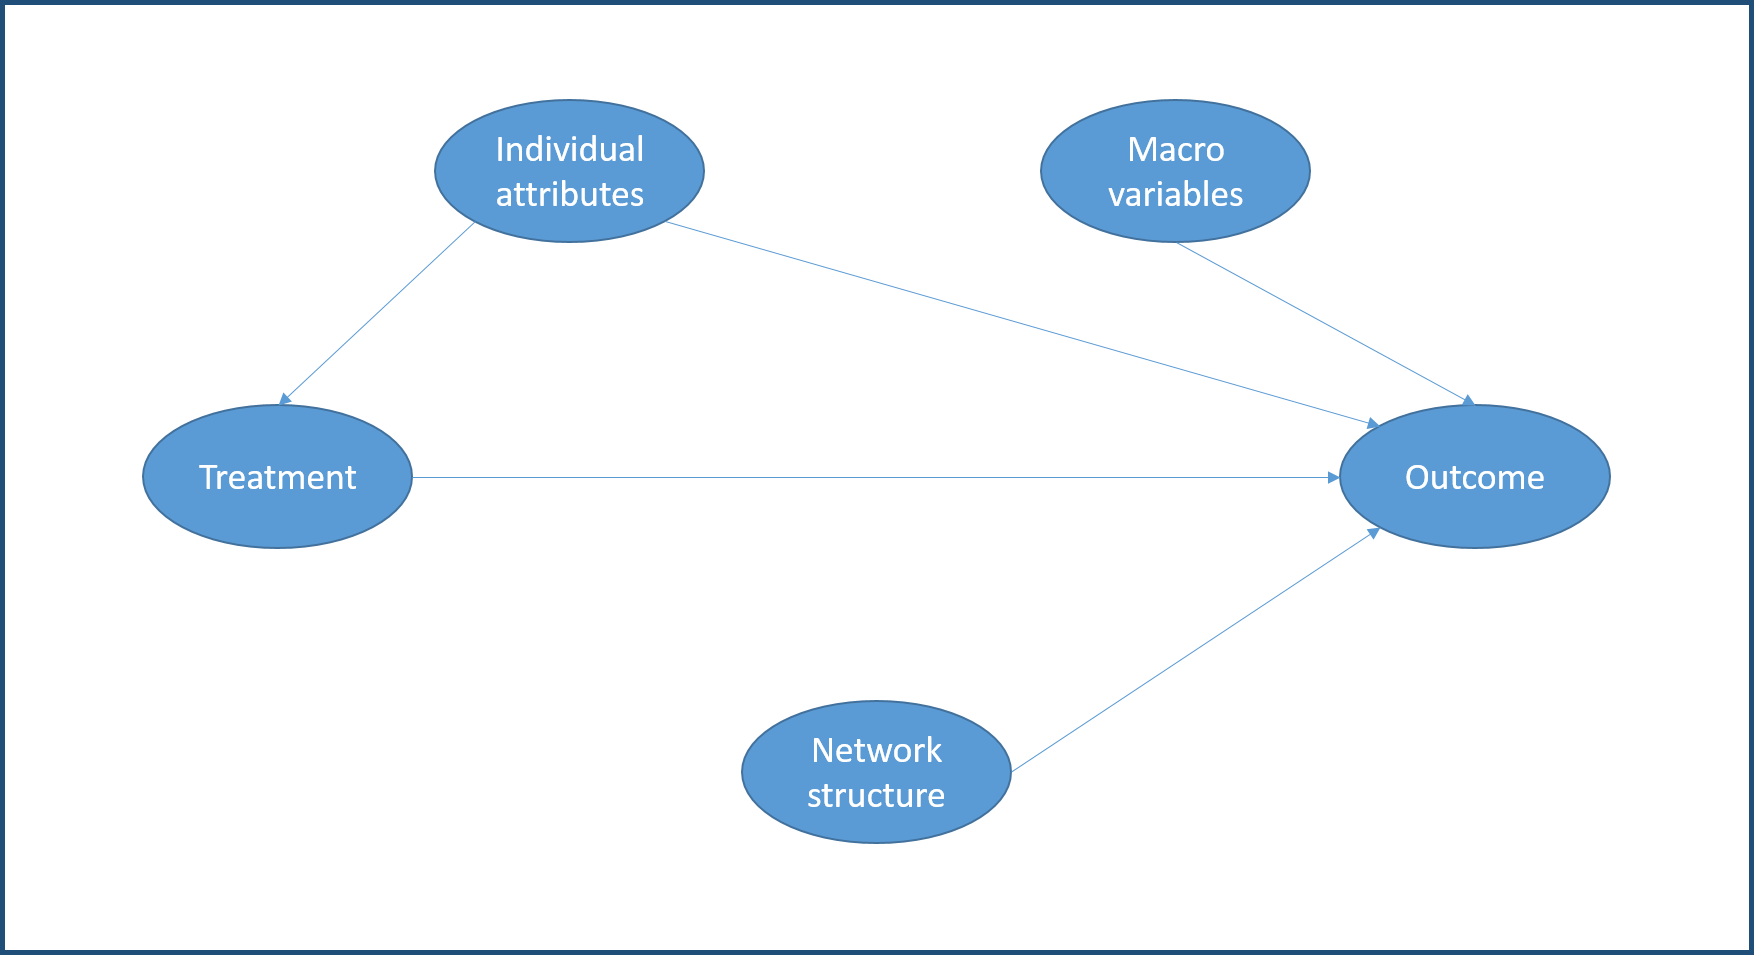
\includegraphics[scale=0.8]{Individual_structure.png}
\end{figure}
	
\centering
\begin{figure}
\centering
\caption{\small \textbf{Network plot}: This is a simple illustration showing how the treatment assignment in the neighborhood of each control unit can impact the spillover treatment effect it may receive. T indicates treated unit and C indicates control}
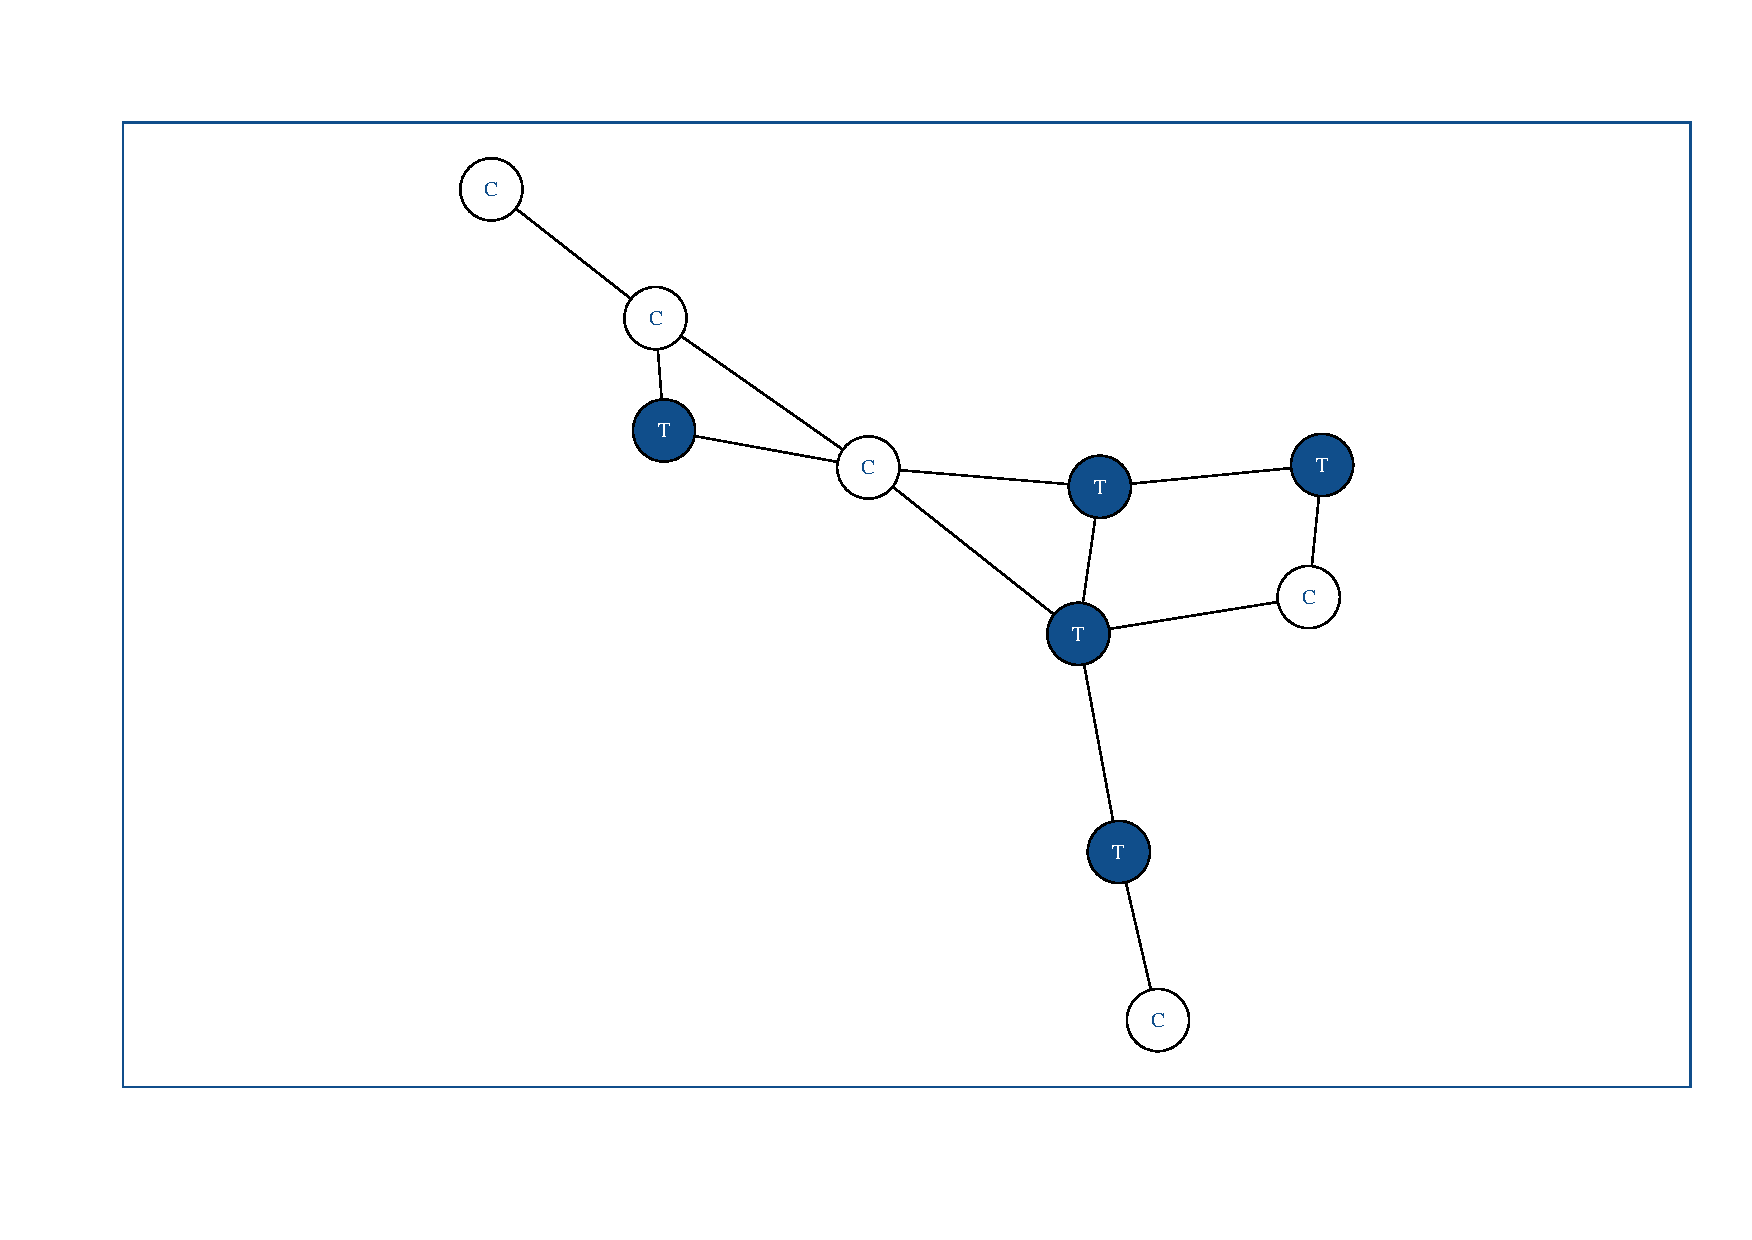
\includegraphics[scale=0.9]{Dummy_network.pdf}
\end{figure}	
	
	
	
	\end{block}
	

\end{column}		
	\begin{column}{\onecolwidd}
	
	\begin{block}{Existing Approaches}
		\begin{rmfamily}
	
	{\Large \textbf{Bowers et. al. method:}}\\
	\citealt{bowers2012reasoning} proposed a method for modeling and testing for spillover effects in network setup.
	

	\begin{itemize}
	
	\item Assume the "sharp null hypothesis of no effects" i.e. the treatment assignment has no effect on any unit
	\vspace*{.1in}
	\item Specify the causal model which describes the change in potential outcomes when treatment assignment changes from \textbf{u} to \textbf{w}; $\mathcal{H}(y_{i, \textbf{u}}, \textbf{w}, \theta)$
	\vspace*{.1in}
	\item Potential outcomes from the causal model must be mapped to observed outcomes $y_z$. Treatment assignment in the experiment (\textbf{z}) must be mapped to the uniformity trial ($\mathcal{H}(y_{\textbf{z}}, \textbf{0}, \theta) = \textbf{y}_0$) which is based on the baseline condition of no-treatment assignment i.e. every unit is a control unit
	\vspace*{.1in}	
	\item Test statistic $\mathcal{T}$ should be a small value when distribution of treated and control outcomes in the adjusted data are similar, and a large value when distributions are dissimilar. We need a sensitive measure to account for similarity on not just the center but also higher-order moments of a distribution. Bowers et. al. recommend the Kolmogorov-Smirnov (KS) test statistic
	\vspace*{.1in}
	\item Assume that treatment only spreads through edges and the spillover effect only depends on the number of neighbours treated. Spillover effect modeled using a growth curve $\beta + (1-\beta)e^{-\tau^2\textbf{z}^T\textbf{S}}$
	\vspace*{.1in}
	\item Generate the distribution of test statistic under our hypothesis. The exact distribution is specified by computing $t_k = \mathcal{T} (\textbf{y}_0, \textbf{Z}_k)$ for each $\textbf{Z}_k \in \Omega$. Alternatively, we can use sampling methods and limit theorems to estimate the distribution from data.
	\vspace*{.1in}
	\item p-value calculated using $\frac{\sum_{k=1}^{abs(\Omega)} I(x_i  > t_k)}{abs(\Omega)}$
	\vspace*{.1in}	
	\end{itemize}

\hspace{2cm}

	{\Large \textbf{Coppock method}}\\
	\citealt{coppock2014information} extends the Bowers method of inference using the New Mexico Legislator experiment conducted by \citealt{butler2011can}. Coppock uses ideological similarity scores in the adjacency matrix, and models the direct treatment effect and spillover occurring through the network.
	
	\end{rmfamily}
	\end{block}
	
	\hspace{2cm}
						
	
	\begin{block}{Proposed extensions}
	\begin{rmfamily}

	We would like to extend this methodology along the following dimensions:
	
	\begin{itemize}
	\item Diffusion of treatment effect along a network will depend on the neighborhood of control units. We will consider various models that consider the following aspects: (tabulated below)
	
	\begin{itemize}
	\item Distance from the nearest treated node
	\item Number/proportion of treated neighbors
	\item Form of spread (linear or non-linear)
	\end{itemize}
	
	\vspace*{.1in}
	\item Consider other legislator networks depending on geographical proximity and co-sponsorship
	\vspace*{.1in}
	\item Consider additional test statistics such as the Anderson-Darling test and other tests mentioned in \citep{rosenbaum2012interference} (Mann-Whitney U test, Control Median test etc.)
	\vspace*{.1in}
	\end{itemize}	

	\end{rmfamily}						
	\end{block}
	
	\begin{rmfamily}						
	\begin{table}
        	\begin{tabular}{lrrrr}\toprule
            &\multicolumn{2}{c}{\textbf{Distance < 5}}&\multicolumn{2}{c}{\textbf{Distance > 5}}
            \\\cmidrule(r){2-3}\cmidrule(r){4-5}
            &Linear&Non-linear&Linear&Non-linear\\\midrule
            Number of treated neighbors    & 1 & 2
                    & 5 & 6\\
            Proportion of treated neighbors   & 3 & 4
                    & 7 & 8
            \\\bottomrule
        	\end{tabular}
        	\caption{Possible models}\label{Tab2}
	\end{table}
	\end{rmfamily}						
	\end{column}
	
	
	%Third column
	\begin{column}{\onecolwidd}
	
	\begin{block}{Data}
	\begin{rmfamily}
	
	The Senate Bill 24 was proposed in the New Mexico state legislature during a special session in 2008. Bill proposed to return a projected budget surplus to taxpayers in form of a rebate. 35 out of the 70 legislators received estimates of support within their constituencies, using matched pair randomization (treatment). Their final vote choice was noted (outcome). Below we see the three possible network structures connecting the legislators:
	
	\hspace{2cm}
	\begin{figure}
	\centering
	\begin{tabular}{cc}
	{\bf Geographic Network} & {\bf Committee Network (>1 in common)}\\
	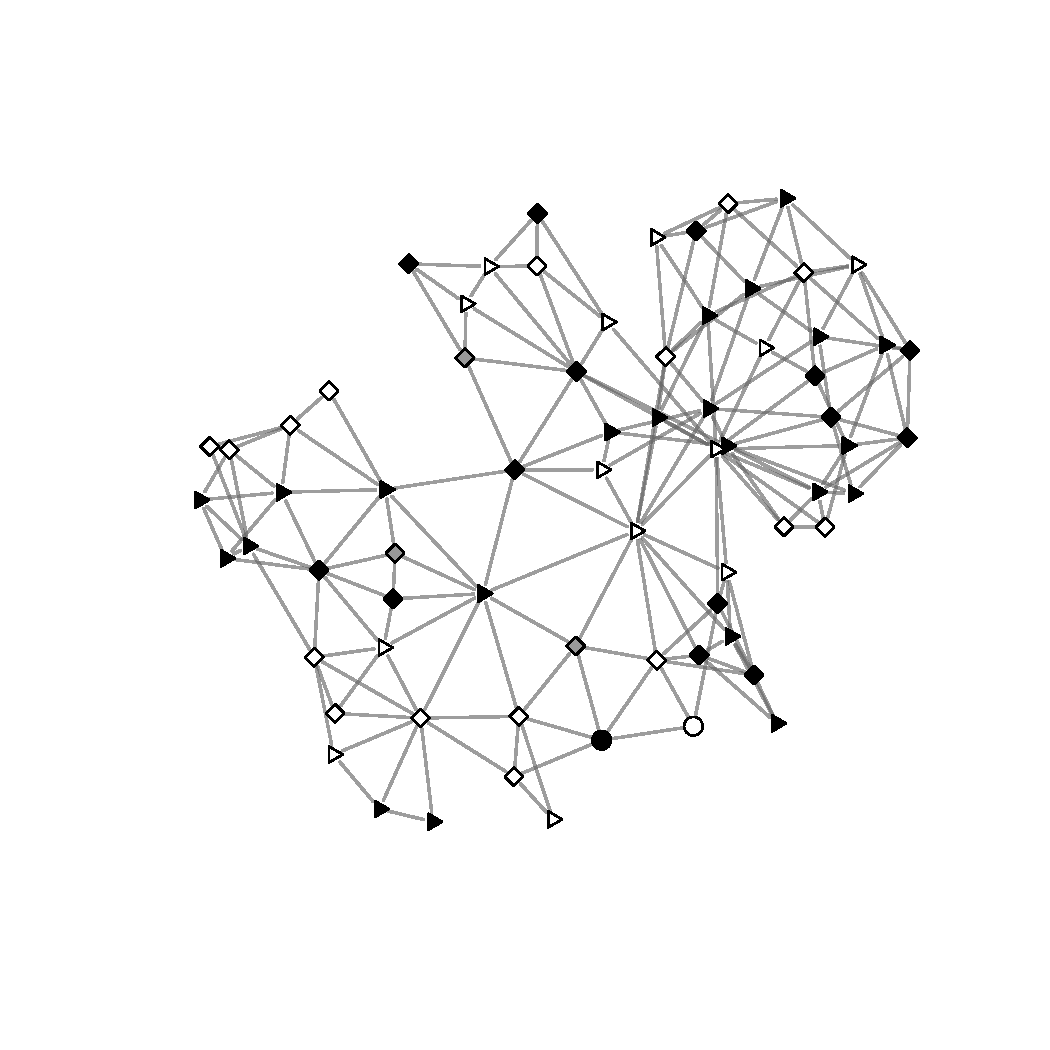
\includegraphics[scale=0.9, clip=true,trim =2cm 2cm 2cm 2cm ]{coppock_geographic_net.pdf} & 						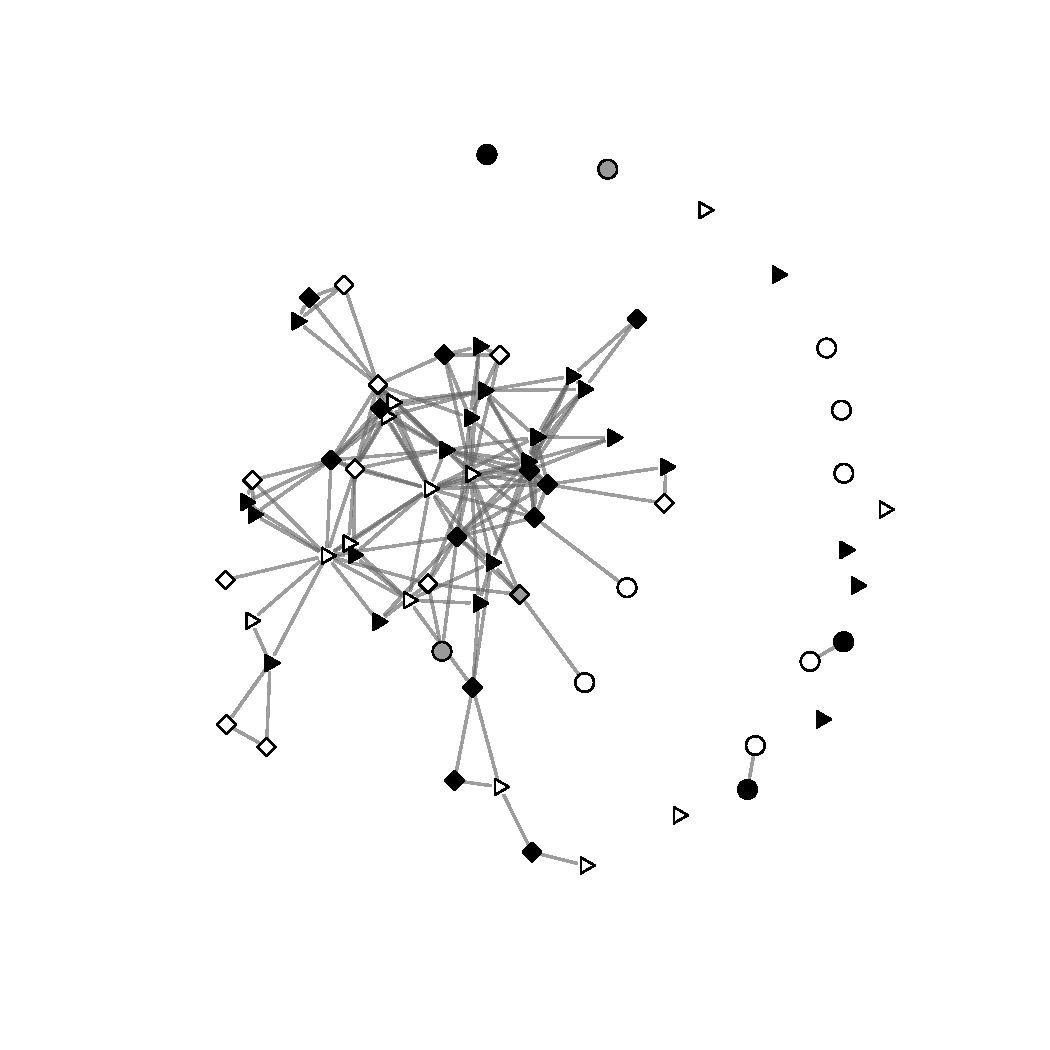
\includegraphics[scale=0.9, clip=true,trim =2cm 2cm 2cm 2cm]{nm_committee_net.pdf} \\ 
	\end{tabular}
	{\bf Ideological Network (top 5\%)} \\
	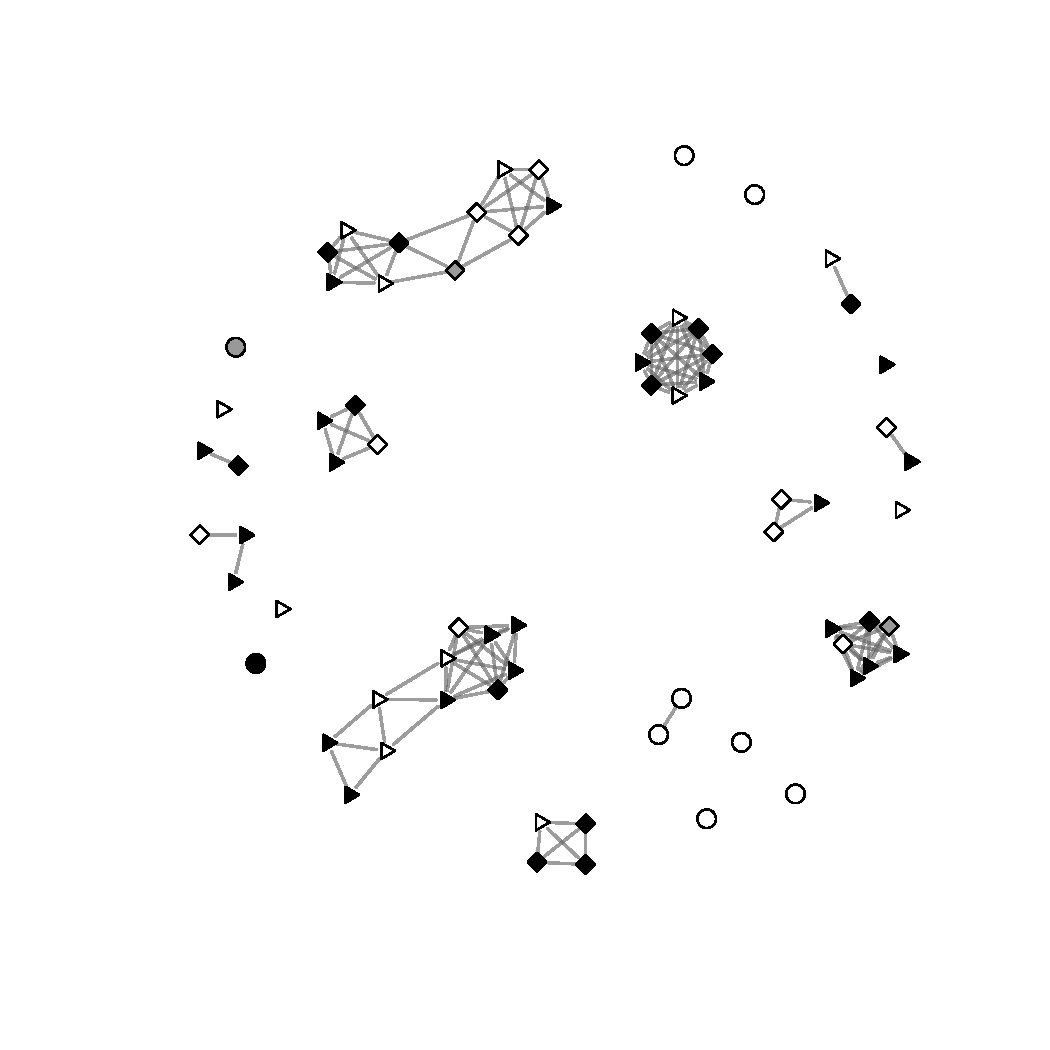
\includegraphics[scale=0.9, clip=true,trim =2cm 2cm 2cm 2cm]{coppock_ideological_net.pdf}
	\caption{Different networks among New Mexico legislators. Colors denote outcome: black means voted with district, gray means abstained, white means voted against. Shape denotes treatment status. Triangles are treated. Squares are adjacent to treated. Circles are isolated from treatment}
	\label{fig:nh-nets}
	\end{figure}

	\end{rmfamily}						
	\end{block}
	

	\begin{block}{Replication}
	\begin{rmfamily}
	
	The figure below contains p-values for a model using ideological similarity scores to explain the spillover of treatment effect. Direct effects are on the X-axis and indirect effects on Y-axis. A p-value here indicates the proportion of simulated test statistic lesser than the observed test statistic. Therefore, a higher p-value indicates support for evidence of spillover effect. Direct and indirect effect values are linear.


	\begin{figure}

	\centering
	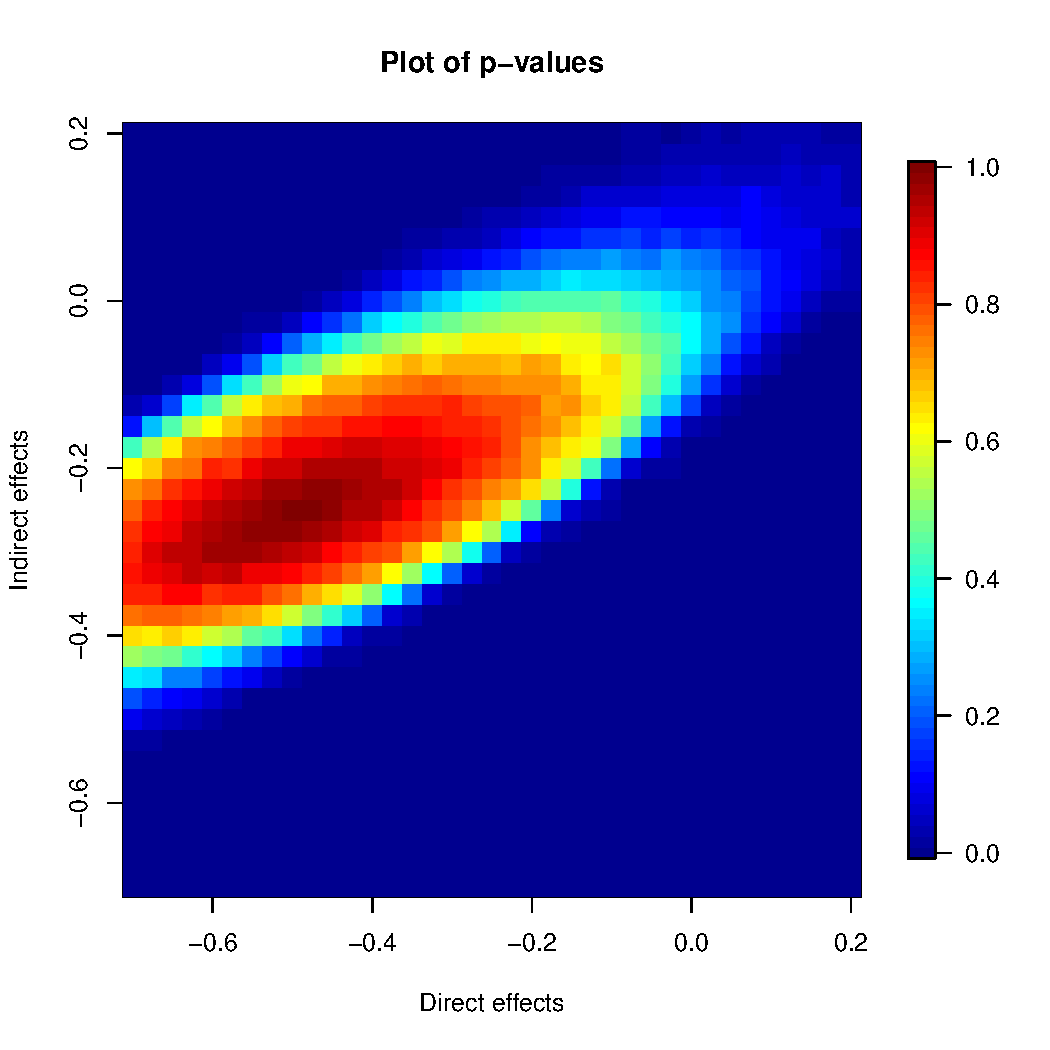
\includegraphics[scale=1]{pvalues_figure.pdf}
	\caption{p-values using Coppock model}
	\end{figure}

	\end{rmfamily}						
	\end{block}
	\end{column}


\begin{column}{\onecolwidd}
\begin{block}{Extension}
	\begin{rmfamily}
	
	We extend the Coppock model using a separate network structure. We use ideological scores and create an adjacency matrix based on whether a particular legislator is one of the k nearest neighbors. We consider values 3, 5, 8 and 12 for k.
	
	\hspace{2cm}
	\begin{figure}
	\centering
	\begin{tabular}{cc}
	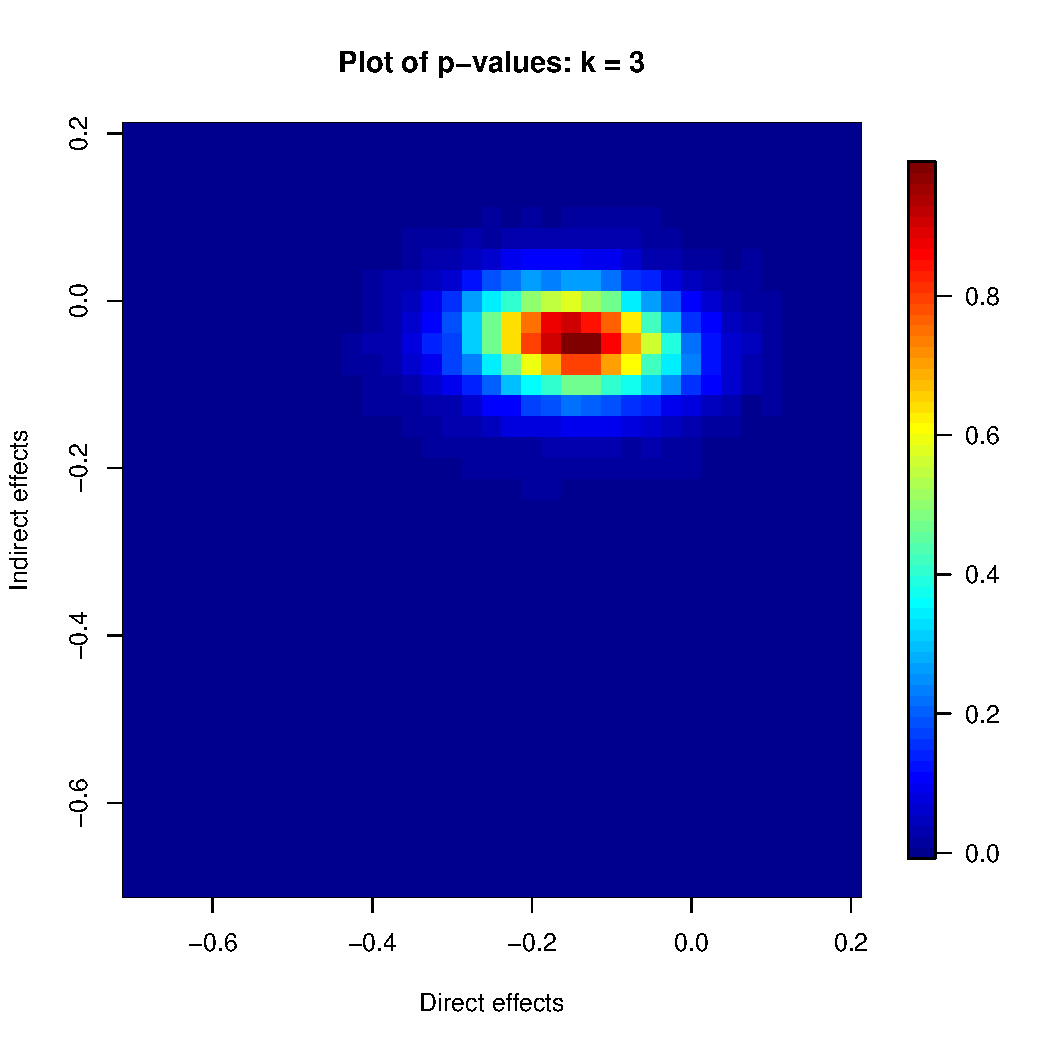
\includegraphics[scale=0.8]{pvalues_figure_3nn.pdf} &
	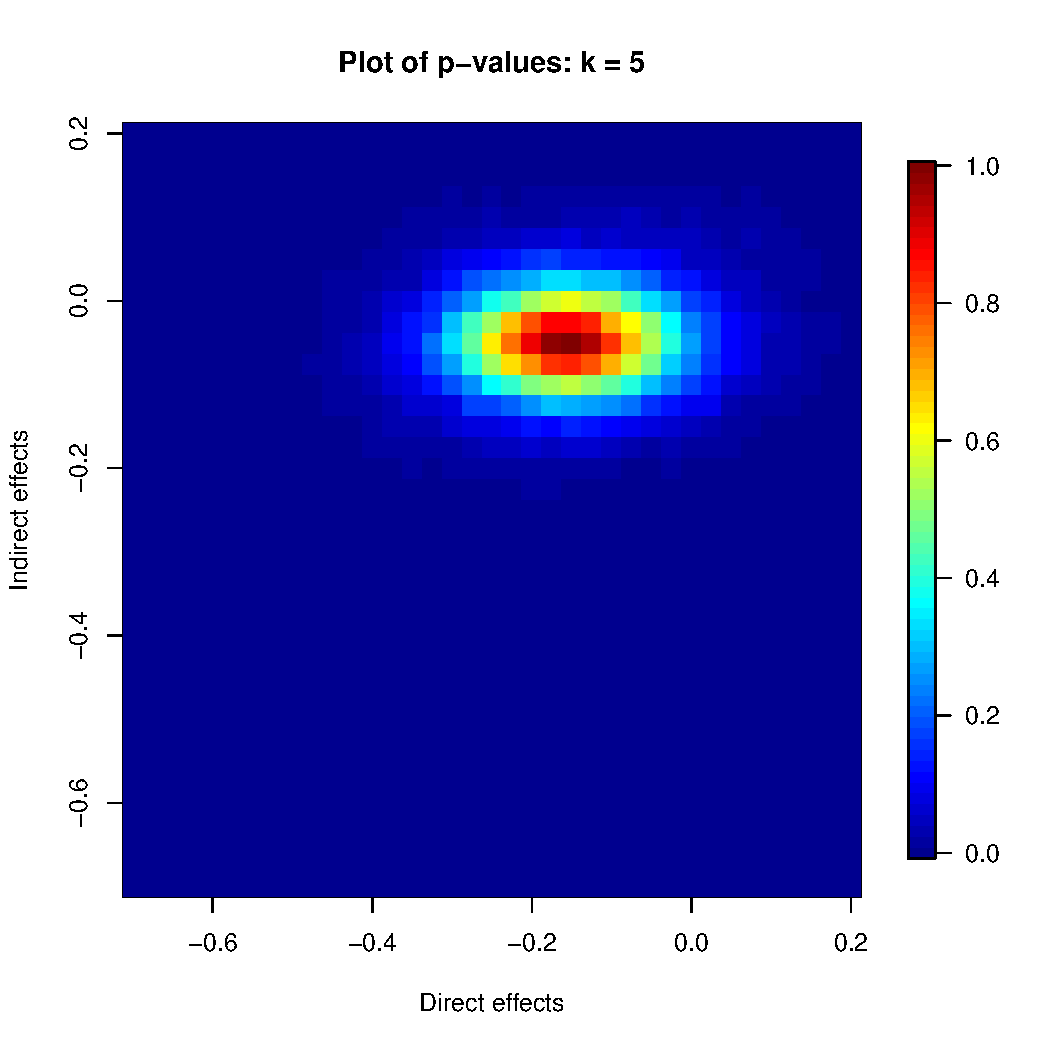
\includegraphics[scale=0.8]{pvalues_figure_5nn.pdf} \\ 
	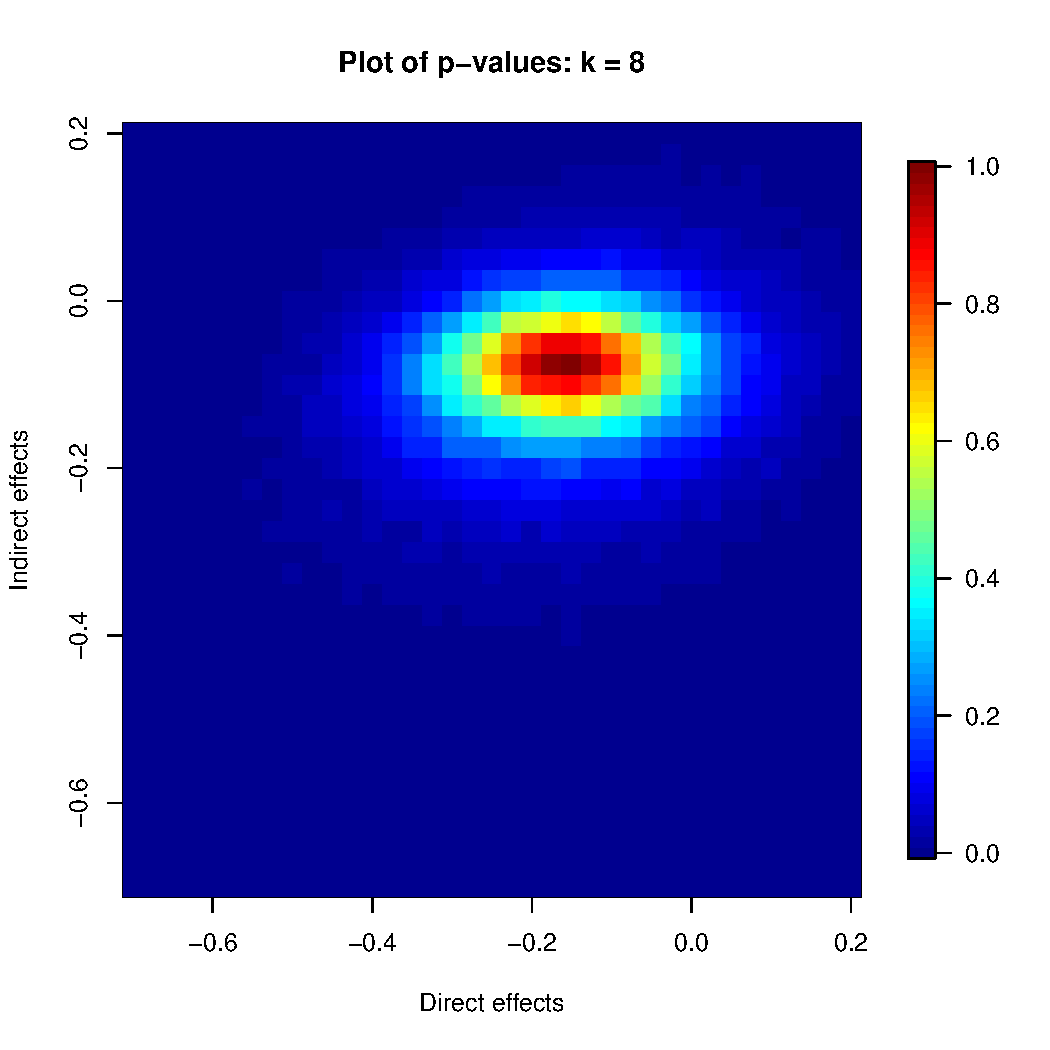
\includegraphics[scale=0.8]{pvalues_figure_8nn.pdf} &
	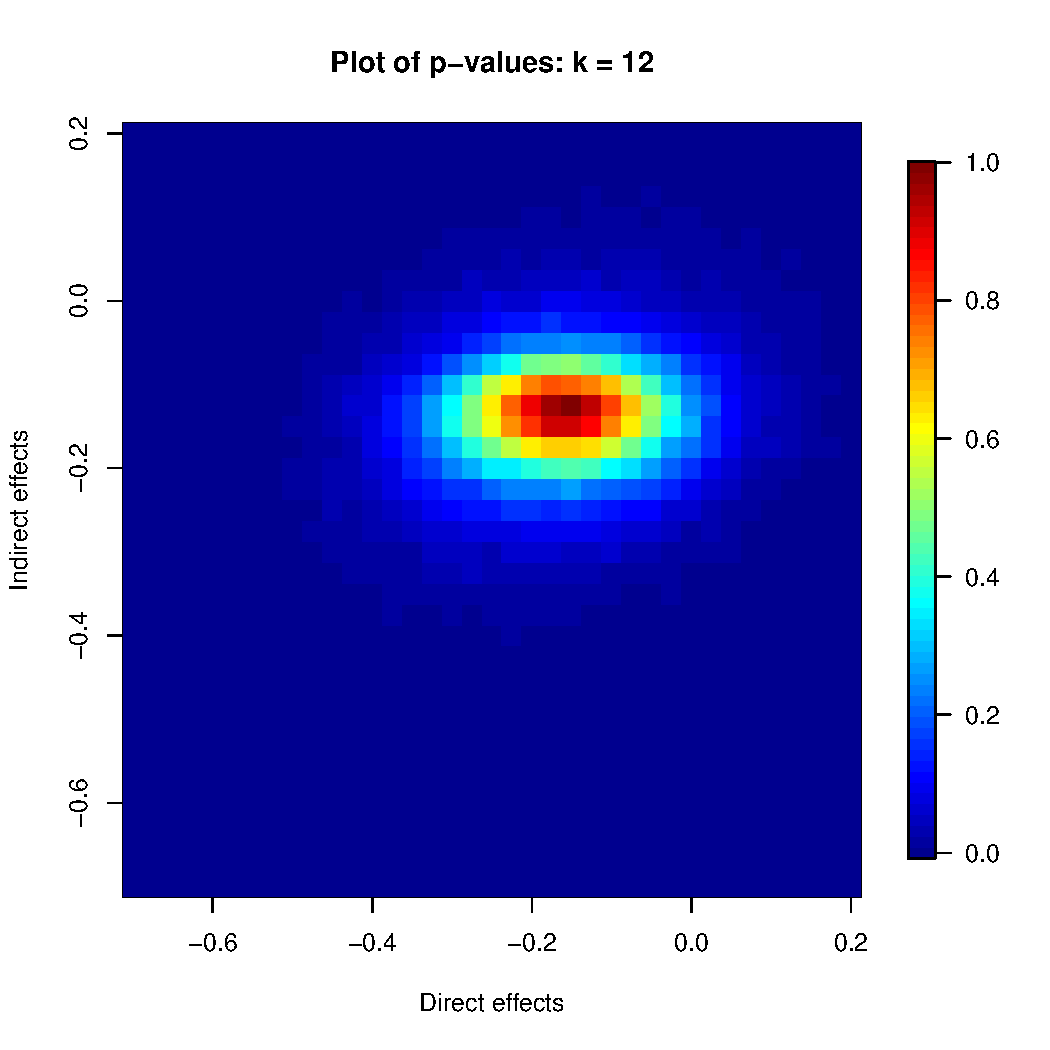
\includegraphics[scale=0.8]{pvalues_figure_12nn.pdf} \\ 
	\end{tabular}
	\caption{p-values using nearest ideological neighbors. k is the number of neighbors considered}
	\end{figure}
	
	\hspace{2cm}
	Under the new specification, the highest p-value moves closer to zero, for both direct and indirect effects. In the original setup, it is -0.45 for direct effects and -0.25 for indirect effects.
		
	\end{rmfamily}						
	\end{block}
	

	\begin{block}{References}
	\bibliographystyle{apsr}
	\bibliography{poster}
	\end{block}	
	
	
	
	
	
	\end{column}
	
	

		
	\end{columns}
	
	
	%\vspace{-0.55in} % adjust to put footer in correct place
	\hspace*{.5in} \begin{beamercolorbox}[wd=50.75in,colsep=0.15cm]{cboxb}\end{beamercolorbox}
	%\vspace{-1.5cm}
	
	\begin{columns}
		
		% UCI logo here
%		\begin{column}{0.23\paperwidth}

		
%			\begin{center}
%				\begin{figure}
%					\includegraphics[scale=2]{wordmark2.jpg}
%			 	\end{figure}
%			\end{center}
			
%		\end{column}
		
%		\begin{column}{1in}
		
%		\end{column}
		
		\begin{column}{0.25\paperwidth}

	\centering
		\begin{tabular}{cc}

 \begin{minipage}{6.5in}
 \bigskip
This material is based on work supported by the National Science Foundation under IGERT Grant DGE-1144860, Big Data Social Science.


\end{minipage}

& 
\begin{minipage}{2.5in}
\bigskip
\includegraphics[scale=.21]{NSF_logo.png}
\end{minipage}
\end{tabular}
			
		\end{column}
		
		\vspace{1cm}
	
	\end{columns}
	
	
	

\end{frame}

\end{document}
